\documentclass[12pt]{article}

\usepackage{scicite,times,graphicx,float,hyperref}
\usepackage[skip=0pt]{caption}
\usepackage[utf8]{inputenc}
\usepackage{enumitem}
\usepackage{booktabs}

%%%%%%%%%%%%%%%%%%%%%%%%%%%%%%%%%%%%%%%%%%%%%%%%%%%%%%%%%%%%%%%%%%%%%%%%%%% PREAMBLE %%%%%%%%%%%%%%%%%%%%%%%%%%%%%%%%%%%%%%%%%%%%%%%%%%%%%%%%%%%%%%%%%%%%%%%%%%%

\topmargin -1.0cm
\oddsidemargin 0.0cm 
\textwidth 16cm 
\textheight 23cm
\footskip 1.0cm

\newenvironment{sciabstract}{%
\begin{quote} \bf}
{\end{quote}}

\newcounter{lastnote}
\newenvironment{scilastnote}{%
  \setcounter{lastnote}{\value{enumiv}}%
  \addtocounter{lastnote}{+1}%
  \begin{list}%
  {\arabic{lastnote}.}
  {\setlength{\leftmargin}{.22in}}
  {\setlength{\labelsep}{.5em}}
}
{\end{list}}

\title{Final Report on:\\Pretix Redundant Operation} 

\author
{Filipe Pires [85122], João Alegria [85048]\\
\\
Computational Infrastructures Management\\
\normalsize{Department of Electronics, Telecommunications and Informatics}\\
\normalsize{University of Aveiro}\\
} 

\date{\today{}}

%%%%%%%%%%%%%%%%%%%%%%%%%%%%%%%%%%%%%%%%%%%%%%%%%%%%%%%%%%%%%%%%%%%%%%%%%%%% REPORT %%%%%%%%%%%%%%%%%%%%%%%%%%%%%%%%%%%%%%%%%%%%%%%%%%%%%%%%%%%%%%%%%%%%%%%%%%%%

\begin{document}

\baselineskip18pt

\maketitle

\section*{Introduction} \label{introduction} %%%%%%%%%%%%%%%%%%%%%%%%%%%%%%%%%%%%%%%%%%%%%%%%%%%%%%%%%%%%%%%%%%%%%%%%%%%%%%%%%%%%%%%%%%%%%%%%%%%%%%%%%%%%%%%%%%%

This report aims to describe the work developed for the final phase of the practical assignment of the discipline of Computational Infrastructures
Management \cite{assign} from the Msc. degree in Informatics Engineering of the University of Aveiro at the Department of Electronics, Telecommunications and
Informatics.
It is assumed that the reader has knowledge about the previous report, and it is here included:
the characterization of the service level agreements for each service;
the description of the load balancing mechanisms among software components;
the redundancy strategy;
the listing of metrics and computational resources monitored, along with the respective defined alarms;
and other relevant aspects such as horizontal scalability and component fault tolerance.

The service provided is Pretix, an online shop, box office and ticket outlet already successfully used by other service providers for conferences, festivals,
exhibitions, workshops and more.
The previously delivered work focused on the product presentation, distributed installation, and resource and performance analysis.
All code developed is publicly accessible in our GitHub repository:

\url{https://github.com/FilipePires98/GIC}.

% \cite{pretix} \cite{rami.io} 
% \cite{pretixdoc} \cite{pretixgit}
% \cite{docker} \cite{django} \cite{gunicorn} \cite{nginx}
% \cite{pretix_img}
% \cite{postgresql} \cite{redis} \cite{pgpool} \cite{haproxy}
% \cite{ansible}

% \texttt{java -cp <userdir>/build/classes fi.FarmInfrastructure}

% \vspace{-10pt}
% \begin{itemize}[noitemsep]
%   \item ...
% \end{itemize}
% \vspace{-10pt}

% \vspace{-10pt}
% \begin{enumerate}[noitemsep]
%   \item ...
% \end{enumerate}
% \vspace{-10pt}

% \begin{figure}[H]
%   \centering
%   \begin{minipage}{\textwidth}
%     \centering
%     \includegraphics[width=\linewidth]{img/.....png}
%   \end{minipage}%
%   \caption{...}
%   \label{...}
% \end{figure} 

% \begin{figure}[H]
%   \centering
%   \begin{minipage}{\textwidth}
%     \centering
%     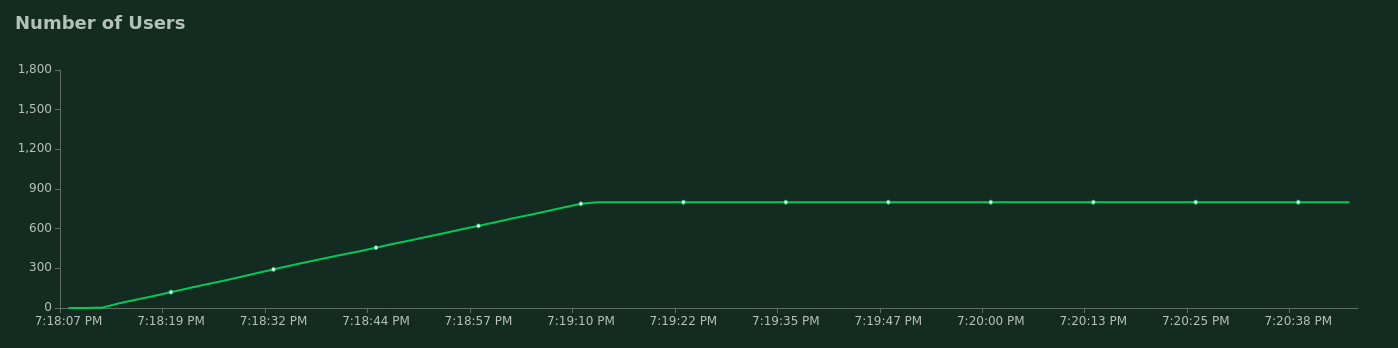
\includegraphics[width=\linewidth]{tests/local/800/number_of_users_1588097887.png}
%   \end{minipage}%
%   \label{fig:LocalTests:number_of_users}
%   \begin{minipage}{\textwidth}
%     \centering
%     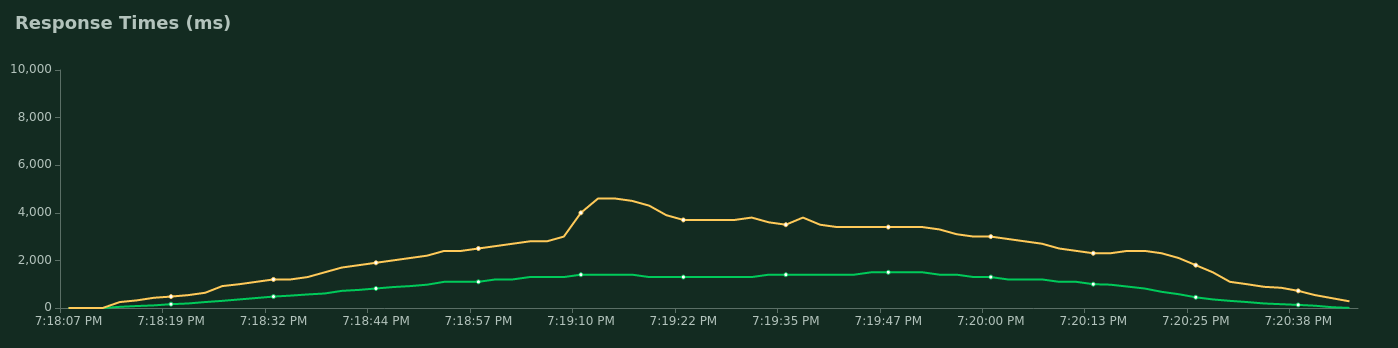
\includegraphics[width=\linewidth]{tests/local/800/response_times_(ms)_1588097887.png}
%   \end{minipage}%
%   \label{fig:LocalTests:response_times_(ms)}
%   \begin{minipage}{\textwidth}
%     \centering
%     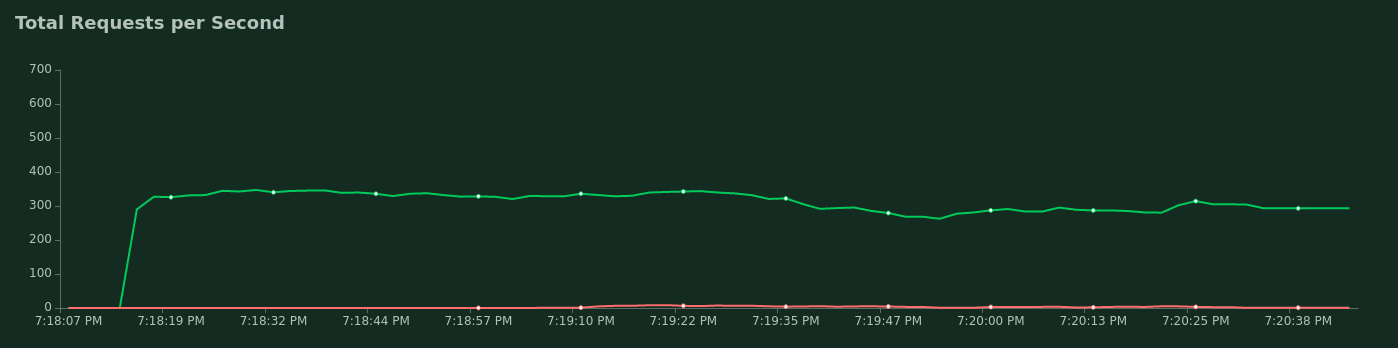
\includegraphics[width=\linewidth]{tests/local/800/total_requests_per_second_1588097887.png}
%   \end{minipage}%
%   \caption{Load tests results with 800 users.}
%   \label{fig:LocalTests:total_requests_per_second}
% \end{figure}
% \vspace{-10pt}

\newpage
\section{System Architecture} \label{architecture} %%%%%%%%%%%%%%%%%%%%%%%%%%%%%%%%%%%%%%%%%%%%%%%%%%%%%%%%%%%%%%%%%%%%%%%%%%%%%%%%%%%%%%%%%%%%%%%%%%%%%%%%%%%%%

\subsection{Infrastructure} \label{architecture.infrastructure} %%%%%%%%%%%%% 

% What is the architecture of the infrastructure deployed?

To provide the Pretix Ticketing Software to the public, it was required to set up an infrastructure containing their Django-based web application, an instance
of a Web Server Gateway Interface (WSGI) hosting the application and of a reverse-proxy for the web application deployment in production mode, as well as a
database management system (DBMS) (where PostgreSQL was used) for handling disk storage and a caching server (where Redis was chosen) for in-memory storage and
asynchronous queuing of tasks.

Our strategy is thoroughly described in the previous report, which already considered minimum redundancy to ensure availability.
It is achieved through the usage of Docker to isolate each component for greater control and easier configuration, and Docker Swarm for the orchestration of
the entire infrastructure.
Nevertheless, as it was a still primitive solution, naturally several upgrades were applied, mostly internally to each container.
The latest architecture is visually presented in Figure \ref{fig:InfrastructureArchitecture}.
This solution considers quality attributes whose assurance is described in the sections below.

\begin{figure}[H]
  \centering
  \begin{minipage}{.85\textwidth}
    \centering
    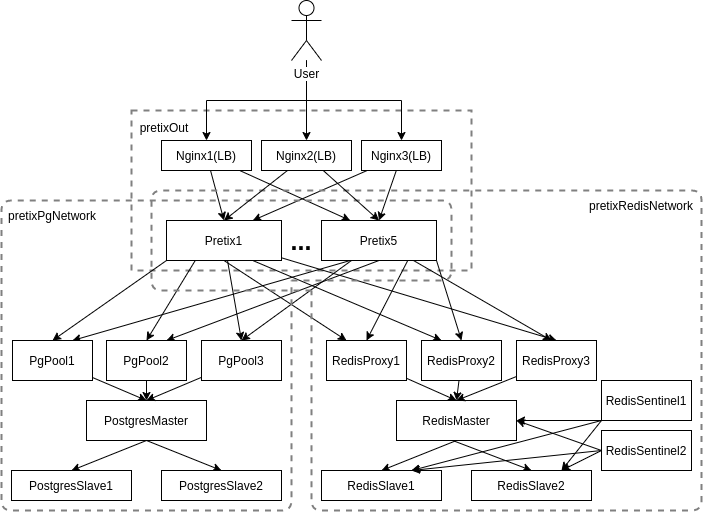
\includegraphics[width=\linewidth]{diagrams/InfrastructureArchitecture.png}
  \end{minipage}%
  \caption{Infrastructure architecture diagram deployed in Docker Swarm.}
  \label{fig:InfrastructureArchitecture}
\end{figure}

\subsection{Load Balancing} \label{architecture.loadbalancing} %%%%%%%%%%%%%

% How is load balancing assured?

The knowledge gathered so far regarding the operation of Pretix affirms that user activity peaks are to be expected when in production.
This has many implications and requires the implementation of mechanisms that maximize the infrastructure's efficiency.

With this in mind, we have come up with mechanisms for load balancing based on proxy servers.
These servers, when strategically placed, act as intermediaries for requests seeking resources from the system itself.
This not only reduces the complexity of requests made to our services, but also provides additional benefits with regards to security and load balancing,
as they allow a controlled and intelligent distribution of requests among components.

An NGinX proxy was installed between the end users and the web application.
With the help of Docker Swarm, replicas of both the proxy and the web application were deployed.
This is transparent for the user and it works as if he/she is sending requests to one single access point.

The storage clusters also resort to proxies.
For the PostgreSQL server cluster, we adopted Pgpool-II.
As our database is replicated in master/slave mode, Pgpool is able to take advantage of the replication feature in order to reduce the load on each PostgreSQL server
by evenly distributing queries among available servers and consequently improving the overall throughput.
Pgpool provides other useful features such as connection pooling, where it maintains established connections to the servers and reuses them whenever a new
connection with the same properties comes in, and automated fail over, mentioned in greater detail in section \ref{management.automation}.

For the Redis server cluster, the adopted solution was the well-known HAProxy.
The instances installed spread requests evenly across the Redis cluster.
Here, a master/slave mode was also used, meaning that the proxies interact with master instances that then delegate work among slaves.

Load tests executed during development proved that such additions had a significant impact on the performance of the system.
The usage of networks, seen in Figure \ref{fig:InfrastructureArchitecture}, where the proxies mentioned above are inserted help orchestrating and logically
grouping components.

\subsection{Redundancy} \label{architecture.redundancy} %%%%%%%%%%%%%%%%%%%%

% How is redundancy assured?

In order for us to provide Pretix, it is only required to maintain one instance of each component running.
However, this is highly unadvisable as it susceptible to failure from any point, i.e. if any of the system components fails, the entire system goes down.
This is referred to as a redundancy measure of N.

Ensuring actual redundancy of a system requires at least a measure of N+1, where each component can be replaced by another if required.
In most cases this is achievable through the replication feature of Docker Swarm.
Pretix's stack has K replicas of NGinX, of the Pretix web application, of Pgpool proxy and of HAProxy, where K can be defined on deployment with a value greater than 2.

Redundancy was also the reason why a master/slave mode was adopted on both clusters.
By instantiating 1 master and K slaves, it is possible to fulfill the requirements implicit to N+1 since if any slave fails the others can replace it and if the
master fails a slave is elected the new master.
Fortunately, for the PostgreSQL cluster this reelection process is done automatically, but for the Redis cluster the use of sentinels is required: sentinels
observe the behavior of masters and slaves, detect failures and reassign roles when needed; here we insist on providing N+1 redundancy by having multiple
instances of sentinels as well.

\subsection{Scalability} \label{architecture.scalability} %%%%%%%%%%%%%%%%%%%%%

% How is horizontal scalability assured?

Any project intended to be successful must consider the scalability of the product in the future.
Ours is no exception since, if the ticketing platform becomes popular, the infrastructure must be prepared to respond to greater loads of income traffic.

There were 2 means to ensure scalability: vertical or horizontal.
As we had access to limited computational resources and adding more physical RAM or CPUs was not an option, the only alternative left was to support horizontal scaling.

The idea here is to make possible the deployment of new replicas of any component and integrate them to the existing infrastructure without significant negative
impact on insertion and in a completely transparent way to the users.
This is exactly what we achieved.
Additionally, each component identifies itself to the monitoring server on initialization so that the data related to what is being managed is constantly up-to-date.

Scaling a portion of the stack can be done both manually or in an automated way.
By default we support manual scaling, but we found it was logical to implement automated mechanisms to scale up or down according to the online users and the
resources used.
This was achieved through the monitoring of meaningful metrics collected from each container instance, as we present in section \ref{management.automation}.

\newpage
\section{Infrastructure Management} \label{management} %%%%%%%%%%%%%%%%%%%%%%%%%%%%%%%%%%%%%%%%%%%%%%%%%%%%%%%%%%%%%%%%%%%%%%%%%%%%%%%%%%%%%%%%%%%%%%%%%%%%%%%%%

\subsection{Service Level Agreement} \label{management.sla} %%%%%%%%%%%%%%%

% What are the SLAs defined?

As service providers, we are supposed to fulfill a commitment with our clients, whether it is formally defined or not.
Obviously it is a good practice to elaborate an agreement where particular aspects of the service are agreed between the service provider and the service user -
this is called a Service Level Agreement (SLA).
We describe ours in this section.

Considering the scope of our project, we've defined the following commitment key points:
\vspace{-10pt}
\begin{itemize}[noitemsep]
  \item Pretix is to be provided through web browsers, by accessing a particular address, and it will only be accessible to those within the university's virtual private network.
  \item Its usage is fully dependent on the usability of the Pretix service itself and no complexity should be added by the infrastructure we provide with regards to this.
  \item We are responsible for providing free access to the ticketing platform through our servers and keeping data integrity even when the service is unavailable
  \item The installations hosting our deployment belong to a third party (the university) and thus we are not accountable for possible availability issues related to networking and machine up time.
        Nevertheless, if this is not considered, we ensure an availability of 100\% under normal circumstances and of 70\% for high activity peaks \footnote{Over 50 requests per minute.}, with a maximum response time of 50 seconds for ticket purchasing requests.
  \item No support is guaranteed for issues about features related to the internal implementation of the ticketing software.
\end{itemize}
\vspace{-10pt}

It is worth mentioning that our analysis to the (free version of the) Pretix product showed that the software had strong limitations on maximum load capacity
and response time that, according to the authors, could not be solved through horizontal scaling.

Focusing on the infrastructure itself and the computational resources, we have defined a list of Service Level Objects (SLO) - the metrics to be observed -
representative of the stack's state, and a list of Service Level Indications (SLI) - the thresholds or functions applied to the metric values - that will
help us react to situations where the SLA compliance is threatened.
These SLOs revolve around: memory capacity, operation latency, data transfer throughput, availability percentage, recovery time and reliability.

...

\subsection{Monitoring} \label{management.monitoring} %%%%%%%%%%%%%%%%%%%%%

% How is the infrastructure monitored? 
% SNMP, logs, metrics exporters

\subsubsection{Log Collection}
\subsubsection{Metric Collection}

\subsection{Alerts and Automation} \label{management.automation} %%%%%%%%%%%%%%%%%%%%%

% SLA violation alarms
% How is the provisioning of new elements automated?
% How is the infrastructure fault tolerant? (pgpool automated failover, redis sentinels, SLA violation alarm responses)

...

\newpage
\section{Additional Remarks} \label{remarks} %%%%%%%%%%%%%%%%%%%%%%%%%%%%%%%%%%%%%%%%%%%%%%%%%%%%%%%%%%%%%%%%%%%%%%%%%%%%%%%%%%%%%%%%%%%%%%%%%%%%%%%%%%%%%%%%%%%

\subsection{Pretix Quickstart} \label{remarks.quickstart} %%%%%%%%%%%%%%%%%

% quickstart script

During development, a need for a faster basic setup of Pretix emerged for debugging purposes.
As many of our tests assumed the existence of organizers and events already inserted on the databases, each time these had to be cleared the objects had to be
manually created before proceeding with some implementation process.

In order to respond to this need, we developed a Python script capable of completely dispose of the manual labour.
This script, which we called \texttt{quickstart.py} and placed under a dedicated folder, uses Selenium \cite{selenium} to create an organization inside Pretix,
generate a secret API key for sending REST requests (storing it in a text file), create a default event and prepare it for load testing with Locust.
It also contains configurable variables to personalize its output.

Such quickstart tool was not only found useful for the obvious advantage in development speed it brought to us, but was also considered a good help tool for any
person that wishes to quickly experiment our infrastructure without having to know much about Pretix itself.

\subsection{Documentation} \label{remarks.documentation} %%%%%%%%%%%%%%%%%%

% what documentation was produced?

A great portion of the code we deal with isn't of our authorship, so the documentation it contains is the documentation we get.
Nevertheless, the code we developed has specific purposes and, although usually very much self explanatory due to its nature, should be easy to interpret by any person.
Our goal is to ensure that what we deliver can be easily reused or even continued by other developers.

With this in mind, we made significant efforts on ensuring that all code developed by us followed a common structure with the same coding style.
Also, we made sure all source files have a description of their purpose and relevant information on the first lines, and contain comments on key points of the
code explaining snippets considered of greater complexity/importance.

\subsection{Assignment Contributions} \label{remarks.contributions} %%%%%%%%%

% who did what?

<<<<<<< HEAD
Regarding the work distribution amongst developers, a close-contact strategy was defined where each worked on a cluster component or piece of software according
to a predefined plan.
=======
Regarding the work distribution among developers, a close-contact strategy was defined where each worked on a cluster component or piece of software according
to a predefined plan.
>>>>>>> 733311d3d5d304f0545f0cf5008b0bde8fced17e
The cluster strategy and respective details were decided in conjunction, as well as the key objectives and tasks to be achieved before the final delivery deadline.

Pretix' features were explored by both developers in order to better comprehend the web platform and the REST API.
Then, João focused on the deployment of our solution on the department's infrastructure while Filipe focused on creating and executing the load tests.
The analysis of the results were carefully conducted in conjunction as well, in order to maintain a common knowledge for better workflows.
It is needless to say that bug and error solving was made along the development phase by both developers any time it was required.
Once performance benchmarking and bottleneck identification were completed, this report and the code documentation became our primary concern, with both
contributing equally.

\newpage
\section*{Conclusions} \label{conclusions} %%%%%%%%%%%%%%%%%%%%%%%%%%%%%%%%%%%%%%%%%%%%%%%%%%%%%%%%%%%%%%%%%%%%%%%%%%%%%%%%%%%%%%%%%%%%%%%%%%%%%%%%%%%%%%%%%%%%%

...

\newpage
\begin{thebibliography}{9} %%%%%%%%%%%%%%%%%%%%%%%%%%%%%%%%%%%%%%%%%%%%%%%%%%%%%%%%%%%%%%%%%%%%%%%%%%%%%%%%%%%%%%%%%%%%%%%%%%%%%%%%%%%%%%%%%%%%%%%%%%%%%%%%%%%%%
  \bibliographystyle{Science}

  \bibitem{assign}
  J. P. Barraca,
  \textit{GIC - Report no.2: Simple Product Operation},
  University of Aveiro,
  2019/20.
  \vspace{-10pt}

  \bibitem{pretix}
  \textit{About Pretix},
  \url{https://pretix.eu/about/en/}.
  Pretix.eu,
  retrieved in April 2020.
  \vspace{-10pt}

  \bibitem{rami.io}
  \textit{Welcome to Rami.io},
  \url{https://rami.io/}.
  Rami.io,
  retrieved in April 2020.
  \vspace{-10pt}

  \bibitem{pretixgit}
  \textit{Pretix Code Repository},
  \url{https://github.com/pretix/pretix}.
  GitHub, Inc.,
  retrieved in April 2020.
  \vspace{-10pt}

  \bibitem{pretixdoc}
  \textit{Welcome to pretix' documentation!},
  \url{https://docs.pretix.eu/en/latest/}.
  Pretix.eu,
  retrieved in April 2020.
  \vspace{-10pt}

  \bibitem{docker}
  \textit{Docker Homepage},
  \url{https://www.docker.com/}.
  Docker Inc.,
  retrieved in April 2020.
  \vspace{-26pt}

  \bibitem{pretix_img}
  \textit{pretix/standalone},
  \url{https://hub.docker.com/r/pretix/standalone}.
  pretix,
  retrieved in April 2020.
  \vspace{-10pt}

  \bibitem{django}
  \textit{Meet Django},
  \url{https://www.djangoproject.com/}.
  Django Software Foundation and individual contributors,
  retrieved in April 2020.
  \vspace{-10pt}

  \bibitem{gunicorn}
  \textit{Gunicorn Homepage},
  \url{https://gunicorn.org/}.
  Gunicorn.org,
  retrieved in April 2020.
  \vspace{-10pt}

  \bibitem{nginx}
  \textit{NGinX News},
  \url{https://nginx.org/}.
  NGinX.org,
  retrieved in April 2020.
  \vspace{-10pt}

  \bibitem{postgresql}
  \textit{PostgreSQL: The World's Most Advanced Open Source Relational Database},
  \url{https://www.postgresql.org/}.
  The PostgreSQL Global Development Group,
  retrieved in April 2020.
  \vspace{-10pt}

  \bibitem{redis}
  \textit{About Redis},
  \url{https://redis.io/}.
  Redis Labs,
  retrieved in April 2020.
  \vspace{-10pt}

  \bibitem{pgpool}
  \textit{Welcome to Pgpool-II},
  \url{https://www.pgpool.net/mediawiki/index.php/Main_Page}.
  PgPool Global Development Group,
  retrieved in April 2020.
  \vspace{-10pt}

  \bibitem{haproxy}
  \textit{HAProxy: The Reliable, High Performance TCP/HTTP Load Balancer},
  \url{https://www.haproxy.org/}.
  HAProxy.org,
  retrieved in April 2020.
  \vspace{-10pt}

  \bibitem{locust}
  \textit{Locust, an open source load testing tool},
  \url{https://locust.io/}.
  Locust.io,
  retrieved in April 2020.
  \vspace{-10pt}

  \bibitem{selenium}
  \textit{About Selenium},
  \url{https://www.selenium.dev/about/}.
  Software Freedom Conservancy,
  retrieved in April 2020.
  \vspace{-10pt}

  \bibitem{ansible}
  \textit{Ansible},
  \url{https://www.ansible.com/}.
  Red Hat,
  retrieved in April 2020.

\end{thebibliography}

\clearpage

\end{document}




















